\begin{tikzpicture}[shorten >=1pt,draw=black, x=1cm, y=1 cm,  node distance=0cm]

\draw[use as bounding box, anchor = north west,draw=none] (-2,-4.25) rectangle (9,3.25);
\clip (-2,-4.25) rectangle (9.0,3.25);

%% setup parameters for NN drawing

\tikzstyle{every pin edge}=[<-,shorten <=1pt,thick]
\tikzstyle{neuron}=[circle,fill=black!25,minimum size=0.75cm ,inner sep=0pt, color=black, draw]
\tikzstyle{input neuron}=[neuron, fill=green!25!blue!25];
\tikzstyle{output neuron}=[neuron, fill=green!25!blue!50];
\tikzstyle{hidden neuron}=[neuron, fill=green!50!orange!25];
\tikzstyle{annot} = [text width=2cm, text centered]


%% define coordinate grid 
\def \xfarleft {-1.25}
\def \xleft {-1.0}
\def \xmid {-0.25}
\def \xright {0.5}
\def \ytop {1.0}
\def \ymid {-0.5}
\def \ybot {-1.15}
\def \yphasetwo {-2.0}
\def \xlabeloffset {0.05}
\def \ylabeloffset {0.15}
\def\layersep{3.0}
\def\vlayersep{1.5}



% Draw the input layer nodes
\visible<2->{\node  (ll) at (\xfarleft,\ymid+1.5*\vlayersep) {\small inputs};}
\visible<2->{\node  (ll) at (\xfarleft,\ymid-1.5*\vlayersep) {$x\in\mathbb{R}^{1\times 3}$};}
\foreach \name/\y in {1/\ymid-\vlayersep,2/\ymid,3/\ymid+\vlayersep}{
\visible<2->{\node[input neuron,fill=orange!100 ] (I-\name) at (\xfarleft,\y) {$I_{\name}$};}
}





\foreach \name/\y in {1/\ymid}{
\visible<2->{\path node[hidden neuron] (H-\name) at (\xfarleft+\layersep,\y) {$\sigma$};}
}



% Draw the output layer node
\visible<2->{\node[thick, output neuron] at (\xfarleft+2.0*\layersep,\ymid) (O) {$O$};}



\foreach \source in {1}{
	\visible<2->{\path[thick,->,black] (H-\source) -- (O) ;}}

\visible<2->{\path[thick,->,black,draw] (O.east) -- ([xshift=0.25*\layersep cm]O.east);}

\visible<2->{\node [anchor=west] (l2) at ([xshift=0.25*\layersep cm]O.east) {\small property};}


\foreach \source in {1}{
	\visible<2->{\path[->,black,draw,thick] (H-\source) -- (O) ;}}

\foreach \source in {1}{
		\visible<4->{\path[thick,->,blue] (H-\source) edge node[rectangle, fill=white,fill opacity=0.75,text opacity=1] {$\color{black}\sigma\left(x{\color{blue}w}\right)$} (O) ;}}



\visible<5>{\node[anchor= west, draw, gray,very thick,fill=white] (latt) at (\xmid+4.5,\ymid) {{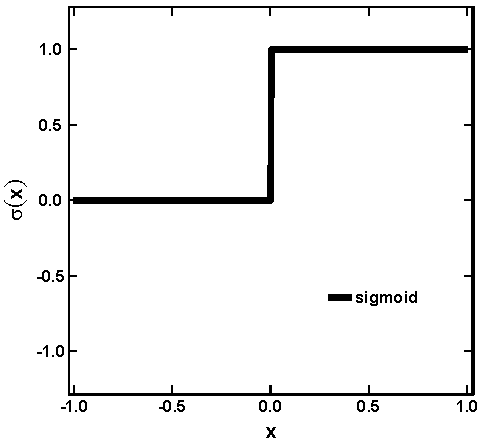
\includegraphics[width= 4.0 cm]{neural_networks/images/act_1}}};}
\visible<6>{\node[anchor= west, draw, gray,very thick,fill=white] (latt) at (\xmid+4.5,\ymid) {{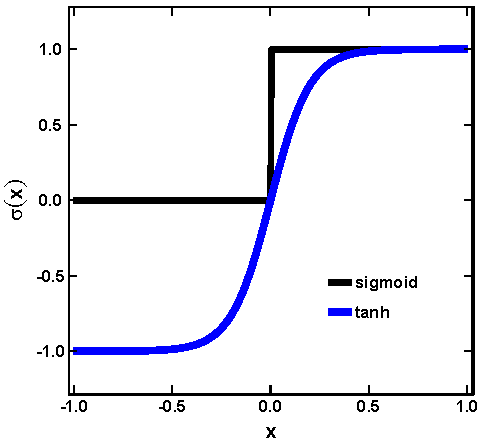
\includegraphics[width= 4.0 cm]{neural_networks/images/act_2}}};}
\visible<7>{\node[anchor= west, draw, gray,very thick,fill=white] (latt) at (\xmid+4.5,\ymid) {{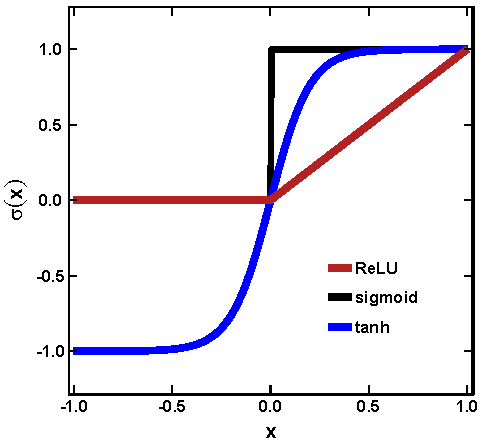
\includegraphics[width= 4.0 cm]{neural_networks/images/act_3}}};}
%
\node[anchor = north west] at (\xmid+1,\ymid-2.0) {
\begin{minipage}{8cm}
\visible<5->{This unit is differentiable as long as $\sigma$ is.}
\vspace{-0.25cm}
\begin{align*}
\only<6>{\frac{\partial O}{\partial {\color{blue}w_1}}&=x_1\sigma'\left(x{\color{blue}w}\right)}
\only<7->{\implies \frac{\partial O}{\partial {\color{blue}w}}  &= x\sigma'\left(x{\color{blue}w}\right)}
\end{align*}
\end{minipage}};
%
%\node[anchor = north west] at (\xmid+0.5,\ymid+2.75) {
%\begin{minipage}{8cm}
%\visible<8->{Note: we do not change anything about $\sigma$, we only tweak the linear combinations of inputs.}
%\end{minipage}};



\foreach \source in {1,2,3}{
\foreach \dest in {1}{     

\visible<2->{\path[thick,->,black] (I-\source) edge[thick] node[] {} (H-\dest) ;}}
}


\foreach \source in {1,2,3}{
\foreach \dest in {1}{     
\visible<3->{\path[thick,->,blue] (I-\source) edge node[rectangle, fill=white,fill opacity=0.5,opacity=1] {{\color{blue}$w_{\source}$}{\color{black}$x_{\source}$}} (H-\dest) ;}}
}




\end{tikzpicture}

